% Options for packages loaded elsewhere
% Options for packages loaded elsewhere
\PassOptionsToPackage{unicode}{hyperref}
\PassOptionsToPackage{hyphens}{url}
\PassOptionsToPackage{dvipsnames,svgnames,x11names}{xcolor}
%
\documentclass[
  letterpaper,
  DIV=11,
  numbers=noendperiod]{scrartcl}
\usepackage{xcolor}
\usepackage{amsmath,amssymb}
\setcounter{secnumdepth}{5}
\usepackage{iftex}
\ifPDFTeX
  \usepackage[T1]{fontenc}
  \usepackage[utf8]{inputenc}
  \usepackage{textcomp} % provide euro and other symbols
\else % if luatex or xetex
  \usepackage{unicode-math} % this also loads fontspec
  \defaultfontfeatures{Scale=MatchLowercase}
  \defaultfontfeatures[\rmfamily]{Ligatures=TeX,Scale=1}
\fi
\usepackage{lmodern}
\ifPDFTeX\else
  % xetex/luatex font selection
\fi
% Use upquote if available, for straight quotes in verbatim environments
\IfFileExists{upquote.sty}{\usepackage{upquote}}{}
\IfFileExists{microtype.sty}{% use microtype if available
  \usepackage[]{microtype}
  \UseMicrotypeSet[protrusion]{basicmath} % disable protrusion for tt fonts
}{}
\makeatletter
\@ifundefined{KOMAClassName}{% if non-KOMA class
  \IfFileExists{parskip.sty}{%
    \usepackage{parskip}
  }{% else
    \setlength{\parindent}{0pt}
    \setlength{\parskip}{6pt plus 2pt minus 1pt}}
}{% if KOMA class
  \KOMAoptions{parskip=half}}
\makeatother

\usepackage{color}
\usepackage{fancyvrb}
\newcommand{\VerbBar}{|}
\newcommand{\VERB}{\Verb[commandchars=\\\{\}]}
\DefineVerbatimEnvironment{Highlighting}{Verbatim}{commandchars=\\\{\}}
% Add ',fontsize=\small' for more characters per line
\usepackage{framed}
\definecolor{shadecolor}{RGB}{241,243,245}
\newenvironment{Shaded}{\begin{snugshade}}{\end{snugshade}}
\newcommand{\AlertTok}[1]{\textcolor[rgb]{0.68,0.00,0.00}{#1}}
\newcommand{\AnnotationTok}[1]{\textcolor[rgb]{0.37,0.37,0.37}{#1}}
\newcommand{\AttributeTok}[1]{\textcolor[rgb]{0.40,0.45,0.13}{#1}}
\newcommand{\BaseNTok}[1]{\textcolor[rgb]{0.68,0.00,0.00}{#1}}
\newcommand{\BuiltInTok}[1]{\textcolor[rgb]{0.00,0.23,0.31}{#1}}
\newcommand{\CharTok}[1]{\textcolor[rgb]{0.13,0.47,0.30}{#1}}
\newcommand{\CommentTok}[1]{\textcolor[rgb]{0.37,0.37,0.37}{#1}}
\newcommand{\CommentVarTok}[1]{\textcolor[rgb]{0.37,0.37,0.37}{\textit{#1}}}
\newcommand{\ConstantTok}[1]{\textcolor[rgb]{0.56,0.35,0.01}{#1}}
\newcommand{\ControlFlowTok}[1]{\textcolor[rgb]{0.00,0.23,0.31}{\textbf{#1}}}
\newcommand{\DataTypeTok}[1]{\textcolor[rgb]{0.68,0.00,0.00}{#1}}
\newcommand{\DecValTok}[1]{\textcolor[rgb]{0.68,0.00,0.00}{#1}}
\newcommand{\DocumentationTok}[1]{\textcolor[rgb]{0.37,0.37,0.37}{\textit{#1}}}
\newcommand{\ErrorTok}[1]{\textcolor[rgb]{0.68,0.00,0.00}{#1}}
\newcommand{\ExtensionTok}[1]{\textcolor[rgb]{0.00,0.23,0.31}{#1}}
\newcommand{\FloatTok}[1]{\textcolor[rgb]{0.68,0.00,0.00}{#1}}
\newcommand{\FunctionTok}[1]{\textcolor[rgb]{0.28,0.35,0.67}{#1}}
\newcommand{\ImportTok}[1]{\textcolor[rgb]{0.00,0.46,0.62}{#1}}
\newcommand{\InformationTok}[1]{\textcolor[rgb]{0.37,0.37,0.37}{#1}}
\newcommand{\KeywordTok}[1]{\textcolor[rgb]{0.00,0.23,0.31}{\textbf{#1}}}
\newcommand{\NormalTok}[1]{\textcolor[rgb]{0.00,0.23,0.31}{#1}}
\newcommand{\OperatorTok}[1]{\textcolor[rgb]{0.37,0.37,0.37}{#1}}
\newcommand{\OtherTok}[1]{\textcolor[rgb]{0.00,0.23,0.31}{#1}}
\newcommand{\PreprocessorTok}[1]{\textcolor[rgb]{0.68,0.00,0.00}{#1}}
\newcommand{\RegionMarkerTok}[1]{\textcolor[rgb]{0.00,0.23,0.31}{#1}}
\newcommand{\SpecialCharTok}[1]{\textcolor[rgb]{0.37,0.37,0.37}{#1}}
\newcommand{\SpecialStringTok}[1]{\textcolor[rgb]{0.13,0.47,0.30}{#1}}
\newcommand{\StringTok}[1]{\textcolor[rgb]{0.13,0.47,0.30}{#1}}
\newcommand{\VariableTok}[1]{\textcolor[rgb]{0.07,0.07,0.07}{#1}}
\newcommand{\VerbatimStringTok}[1]{\textcolor[rgb]{0.13,0.47,0.30}{#1}}
\newcommand{\WarningTok}[1]{\textcolor[rgb]{0.37,0.37,0.37}{\textit{#1}}}

\usepackage{longtable,booktabs,array}
\usepackage{calc} % for calculating minipage widths
\usepackage{caption}
% Make caption package work with longtable
\makeatletter
\def\fnum@table{\tablename~\thetable}
\makeatother
\usepackage{graphicx}
\makeatletter
\newsavebox\pandoc@box
\newcommand*\pandocbounded[1]{% scales image to fit in text height/width
  \sbox\pandoc@box{#1}%
  \Gscale@div\@tempa{\textheight}{\dimexpr\ht\pandoc@box+\dp\pandoc@box\relax}%
  \Gscale@div\@tempb{\linewidth}{\wd\pandoc@box}%
  \ifdim\@tempb\p@<\@tempa\p@\let\@tempa\@tempb\fi% select the smaller of both
  \ifdim\@tempa\p@<\p@\scalebox{\@tempa}{\usebox\pandoc@box}%
  \else\usebox{\pandoc@box}%
  \fi%
}
% Set default figure placement to htbp
\def\fps@figure{htbp}
\makeatother


% definitions for citeproc citations
\NewDocumentCommand\citeproctext{}{}
\NewDocumentCommand\citeproc{mm}{%
  \begingroup\def\citeproctext{#2}\cite{#1}\endgroup}
\makeatletter
 % allow citations to break across lines
 \let\@cite@ofmt\@firstofone
 % avoid brackets around text for \cite:
 \def\@biblabel#1{}
 \def\@cite#1#2{{#1\if@tempswa , #2\fi}}
\makeatother
\newlength{\cslhangindent}
\setlength{\cslhangindent}{1.5em}
\newlength{\csllabelwidth}
\setlength{\csllabelwidth}{3em}
\newenvironment{CSLReferences}[2] % #1 hanging-indent, #2 entry-spacing
 {\begin{list}{}{%
  \setlength{\itemindent}{0pt}
  \setlength{\leftmargin}{0pt}
  \setlength{\parsep}{0pt}
  % turn on hanging indent if param 1 is 1
  \ifodd #1
   \setlength{\leftmargin}{\cslhangindent}
   \setlength{\itemindent}{-1\cslhangindent}
  \fi
  % set entry spacing
  \setlength{\itemsep}{#2\baselineskip}}}
 {\end{list}}
\usepackage{calc}
\newcommand{\CSLBlock}[1]{\hfill\break\parbox[t]{\linewidth}{\strut\ignorespaces#1\strut}}
\newcommand{\CSLLeftMargin}[1]{\parbox[t]{\csllabelwidth}{\strut#1\strut}}
\newcommand{\CSLRightInline}[1]{\parbox[t]{\linewidth - \csllabelwidth}{\strut#1\strut}}
\newcommand{\CSLIndent}[1]{\hspace{\cslhangindent}#1}



\setlength{\emergencystretch}{3em} % prevent overfull lines

\providecommand{\tightlist}{%
  \setlength{\itemsep}{0pt}\setlength{\parskip}{0pt}}



 


\KOMAoption{captions}{tableheading}
\makeatletter
\@ifpackageloaded{caption}{}{\usepackage{caption}}
\AtBeginDocument{%
\ifdefined\contentsname
  \renewcommand*\contentsname{Table of contents}
\else
  \newcommand\contentsname{Table of contents}
\fi
\ifdefined\listfigurename
  \renewcommand*\listfigurename{List of Figures}
\else
  \newcommand\listfigurename{List of Figures}
\fi
\ifdefined\listtablename
  \renewcommand*\listtablename{List of Tables}
\else
  \newcommand\listtablename{List of Tables}
\fi
\ifdefined\figurename
  \renewcommand*\figurename{Figure}
\else
  \newcommand\figurename{Figure}
\fi
\ifdefined\tablename
  \renewcommand*\tablename{Table}
\else
  \newcommand\tablename{Table}
\fi
}
\@ifpackageloaded{float}{}{\usepackage{float}}
\floatstyle{ruled}
\@ifundefined{c@chapter}{\newfloat{codelisting}{h}{lop}}{\newfloat{codelisting}{h}{lop}[chapter]}
\floatname{codelisting}{Listing}
\newcommand*\listoflistings{\listof{codelisting}{List of Listings}}
\makeatother
\makeatletter
\makeatother
\makeatletter
\@ifpackageloaded{caption}{}{\usepackage{caption}}
\@ifpackageloaded{subcaption}{}{\usepackage{subcaption}}
\makeatother
\usepackage{bookmark}
\IfFileExists{xurl.sty}{\usepackage{xurl}}{} % add URL line breaks if available
\urlstyle{same}
\hypersetup{
  pdftitle={Análisis de Supervivencia},
  pdfauthor={Sergio M. Nava Muñoz},
  colorlinks=true,
  linkcolor={blue},
  filecolor={Maroon},
  citecolor={Blue},
  urlcolor={Blue},
  pdfcreator={LaTeX via pandoc}}


\title{Análisis de Supervivencia}
\usepackage{etoolbox}
\makeatletter
\providecommand{\subtitle}[1]{% add subtitle to \maketitle
  \apptocmd{\@title}{\par {\large #1 \par}}{}{}
}
\makeatother
\subtitle{Introducción}
\author{Sergio M. Nava Muñoz}
\date{2025-06-01}
\begin{document}
\maketitle


\section{Introducción al Análisis de
Supervivencia}\label{introducciuxf3n-al-anuxe1lisis-de-supervivencia}

\subsection{Introducción y Objetivos}\label{introducciuxf3n-y-objetivos}

\begin{itemize}
\tightlist
\item
  \textbf{Relevancia de la Supervivencia} en contextos biomédicos,
  industriales y económicos
\item
  \textbf{Objetivos de la sesión}:

  \begin{itemize}
  \tightlist
  \item
    Comprender conceptos clave: tiempo de falla, funciones de
    supervivencia y riesgo
  \item
    Mecanismos de censura y truncamiento
  \item
    Modelos de supervivencia básicos y estimación en R
  \item
    Aplicaciones prácticas con ejemplos de datos reales
  \end{itemize}
\end{itemize}

\subsection{¿Qué es el análisis de
supervivencia?}\label{quuxe9-es-el-anuxe1lisis-de-supervivencia}

\begin{quote}
\textbf{Análisis de Supervivencia}\\
\end{quote}

\begin{quote}
El análisis de supervivencia, también conocido como análisis de
\textbf{tiempo hasta evento}, es un conjunto de técnicas estadísticas
diseñadas para manejar datos censurados y modelar la distribución del
tiempo hasta la ocurrencia de un evento de interés, ver Klein \&
Moeschberger (2003).
\end{quote}

Más precisamente, estudia el \textbf{tiempo transcurrido entre dos
eventos}:

\begin{itemize}
\tightlist
\item
  Un evento de \textbf{inicio}\\
\item
  Un evento de \textbf{fin}
\end{itemize}

\textbf{Símbolo usual}: \(T\)\\
→ Variable aleatoria no negativa que representa el tiempo hasta el
evento.

\textbf{Términos comunes}:

\begin{itemize}
\tightlist
\item
  Tiempo de falla
\item
  Tiempo de vida
\item
  Tiempo de supervivencia
\end{itemize}

\begin{center}\rule{0.5\linewidth}{0.5pt}\end{center}

\subsection{¿Dónde se aplica el análisis de
supervivencia?}\label{duxf3nde-se-aplica-el-anuxe1lisis-de-supervivencia}

\subsubsection{Aplicaciones comunes}\label{aplicaciones-comunes}

\begin{itemize}
\tightlist
\item
  \textbf{Biomédicas}

  \begin{itemize}
  \tightlist
  \item
    Tiempo hasta recaída, muerte, recuperación o aparición de una
    enfermedad.
  \end{itemize}
\item
  \textbf{Industriales}

  \begin{itemize}
  \tightlist
  \item
    Duración de dispositivos, tiempo hasta la primera falla.
  \end{itemize}
\item
  \textbf{Económicas / financieras}

  \begin{itemize}
  \tightlist
  \item
    Tiempo en desempleo, tiempo hasta bancarrota, duración de relaciones
    laborales.
  \end{itemize}
\end{itemize}

\textbf{Nota}: El ``tiempo'' puede medirse en días, semanas, kilómetros,
horas de operación, etc.

\begin{center}\rule{0.5\linewidth}{0.5pt}\end{center}

\subsection{Naturaleza de los datos de
supervivencia}\label{naturaleza-de-los-datos-de-supervivencia}

\begin{itemize}
\tightlist
\item
  Los datos de tiempo a evento son realizaciones de \textbf{variables
  aleatorias no negativas}.
\item
  Pueden ser:

  \begin{itemize}
  \tightlist
  \item
    \textbf{Continuos}: como tiempo en días, semanas, horas.
  \item
    \textbf{Discretos}: como número de visitas o ciclos.
  \end{itemize}
\end{itemize}

\textbf{Ejemplo de variable de interés}:\\
\[
T = \text{Tiempo entre el ingreso al hospital y la recuperación}
\]

\begin{center}\rule{0.5\linewidth}{0.5pt}\end{center}

\subsection{¿Qué se necesita definir para analizar tiempos de
falla?}\label{quuxe9-se-necesita-definir-para-analizar-tiempos-de-falla}

Para interpretar adecuadamente los datos, es necesario:

\subsubsection{1. Evento de origen}\label{evento-de-origen}

→ ¿Desde cuándo empieza a contarse el tiempo?

\subsubsection{2. Escala de medición}\label{escala-de-mediciuxf3n}

→ ¿Cómo se mide el tiempo? (reloj, kilómetros, ciclos)

\subsubsection{3. Evento de fin}\label{evento-de-fin}

→ ¿Qué se considera ``fallo'', ``recuperación'', o ``evento''?

\section{Ejemplos}\label{ejemplos}

\subsection{Ejemplos varios}\label{ejemplos-varios}

\textbf{Ejemplo biomédico -- Ensayo clínico}:

\begin{itemize}
\tightlist
\item
  Evento de origen: entrada del paciente al estudio
\item
  Evento de fin: muerte o recuperación
\item
  Escala: tiempo en semanas
\end{itemize}

\textbf{Ejemplo industrial -- Billetes}:

\begin{itemize}
\tightlist
\item
  Evento de origen: salida a circulación
\item
  Evento de fin: destrucción por deterioro
\item
  Escala: tiempo calendario o número de transacciones
\end{itemize}

\textbf{Ejemplo financiero -- Desempleo}:

\begin{itemize}
\tightlist
\item
  Evento de origen: pérdida de empleo
\item
  Evento de fin: contratación nueva
\item
  Escala: meses sin empleo
\end{itemize}

\begin{center}\rule{0.5\linewidth}{0.5pt}\end{center}

\subsection{Ejemplos de datos de supervivencia en
bioestadìstica}\label{ejemplos-de-datos-de-supervivencia-en-bioestaduxecstica}

A continuación se presentan algunos ejemplos de datos de supervivencia.
Estos ejemplos fueron obtenidos de Klein \& Moeschberger (2003).

\subsubsection{Ejemplo de Duración de la remisión en un ensayo clínico
para leucemia
aguda}\label{ejemplo-de-duraciuxf3n-de-la-remisiuxf3n-en-un-ensayo-cluxednico-para-leucemia-aguda}

\begin{quote}
Duración de remisión de un ensayo clínico para leucemia aguda.
Resultados de un ensayo clínico en donde se quería compara la
efectividad de la droga \(6-MP\) versus placebo en 42 niños con leucemia
aguda. El evento de inicio es remisión parcial de la enfermedad después
de haber sido tratados con la droga prednisone. El evento de fin es
recaída o muerte. La escala de medición es tiempo calendario en meses.
Algunos individuos no presentaron el evento de fin al término del
estudio. Estos casos son marcados con un + y son llamados censurados por
la derecha. Más adelante los veremos con detalle.
\end{quote}

\begin{center}
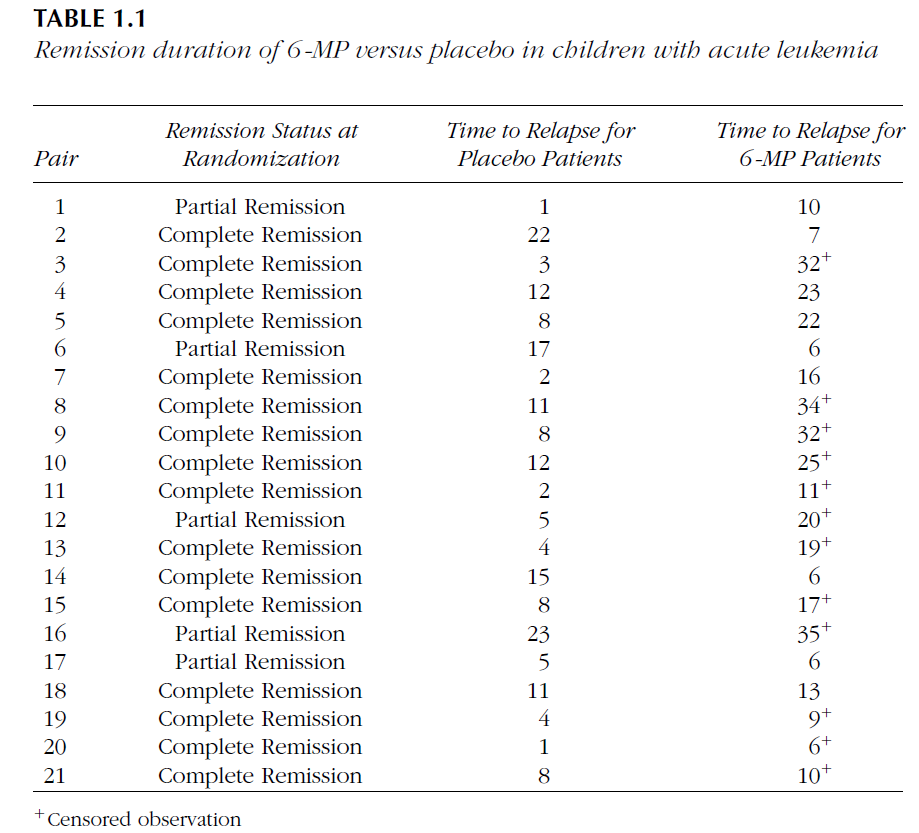
\includegraphics[width=0.4\linewidth,height=\textheight,keepaspectratio]{figura/ejemp1.png}
\end{center}

\begin{center}\rule{0.5\linewidth}{0.5pt}\end{center}

\subsubsection{Ejemplo de Transplante de médula ósea en pacientes con
leucemia.}\label{ejemplo-de-transplante-de-muxe9dula-uxf3sea-en-pacientes-con-leucemia.}

\begin{quote}
Transplante de médula es un procedimiento estándar en pacientes con
leucemia aguda. La recuperación después del transplante es un proceso
complejo. La prognosis para la recuperación puede depender de factores
que se conocen al momento del transplante, como edad y sexo del paciente
y donador, etapa de la enfermedad inicial, tiempo entre el diagnóstico y
el transplante, etc. La prognosis final depende de cómo evoluciona el
paciente después del transplante. Puede generar aversión o rechazo de la
medula transplantada (GVHD), que el conteo de plaquetas se vuelva normal
o desarrollar infecciones, etc. El transplante se considera fracaso
cuando el paciente recae o muere.
\end{quote}

\begin{center}
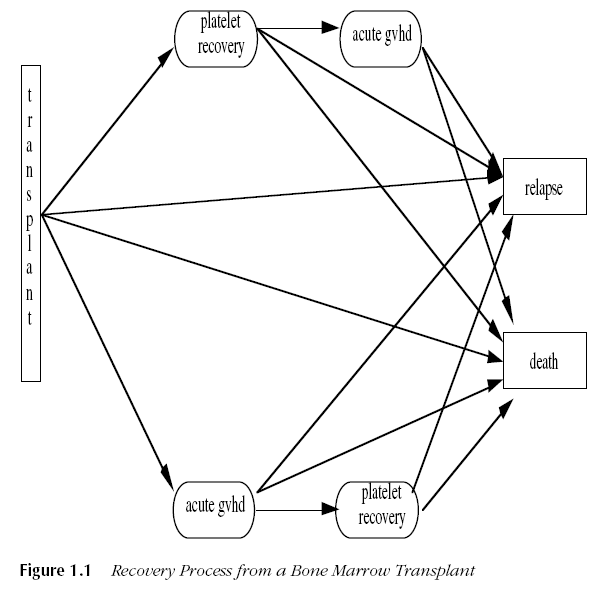
\includegraphics[width=0.4\linewidth,height=\textheight,keepaspectratio]{figura/ejemp2.png}
\end{center}

\begin{center}\rule{0.5\linewidth}{0.5pt}\end{center}

\subsubsection{Ejemplo de Transplante de médula ósea en pacientes con
leucemia.
(cont.)}\label{ejemplo-de-transplante-de-muxe9dula-uxf3sea-en-pacientes-con-leucemia.-cont.}

\begin{figure}

\begin{minipage}{0.50\linewidth}
\begin{center}
\pandocbounded{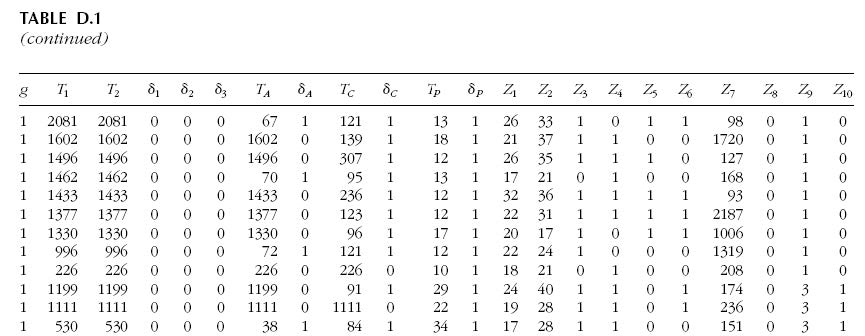
\includegraphics[keepaspectratio]{figura/ejemp2-3.jpg}}
\end{center}
\end{minipage}%
%
\begin{minipage}{0.50\linewidth}
\begin{center}
\pandocbounded{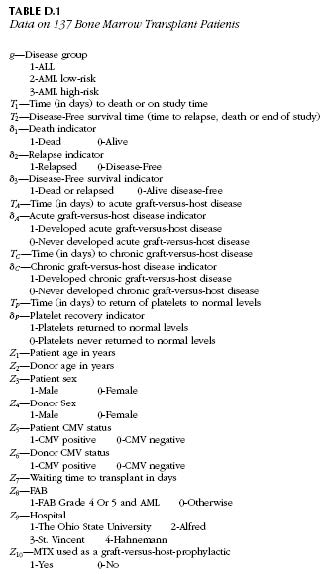
\includegraphics[keepaspectratio]{figura/ejemp2-2.jpg}}
\end{center}
\end{minipage}%

\end{figure}%

\begin{center}\rule{0.5\linewidth}{0.5pt}\end{center}

\subsubsection{Ejemplo Tiempos de muerte de adultos mayores residentes
de un
asilo.}\label{ejemplo-tiempos-de-muerte-de-adultos-mayores-residentes-de-un-asilo.}

\begin{quote}
Channing House es una casa de retiro en California. Datos con las edades
de muerte de 462 individuos (97 hombres y 365 mujeres) que estuvieron en
la residencia durante el periodo de enero de 1964 y julio de 1975. Se
reportó la edad a la muerte o al momento en que se salían del asilo (en
meses) y la edad a la que los individuos entraron al asilo. Estos datos
son un ejemplo de truncamiento por la izquierda que más adelante veremos
con detalle. Un individuo tiene que sobrevivir lo suficiente para estar
en edad de entrar al asilo. Individuos que mueren previamente a la edad
de retiro son excluidos del estudio.
\end{quote}

\begin{center}
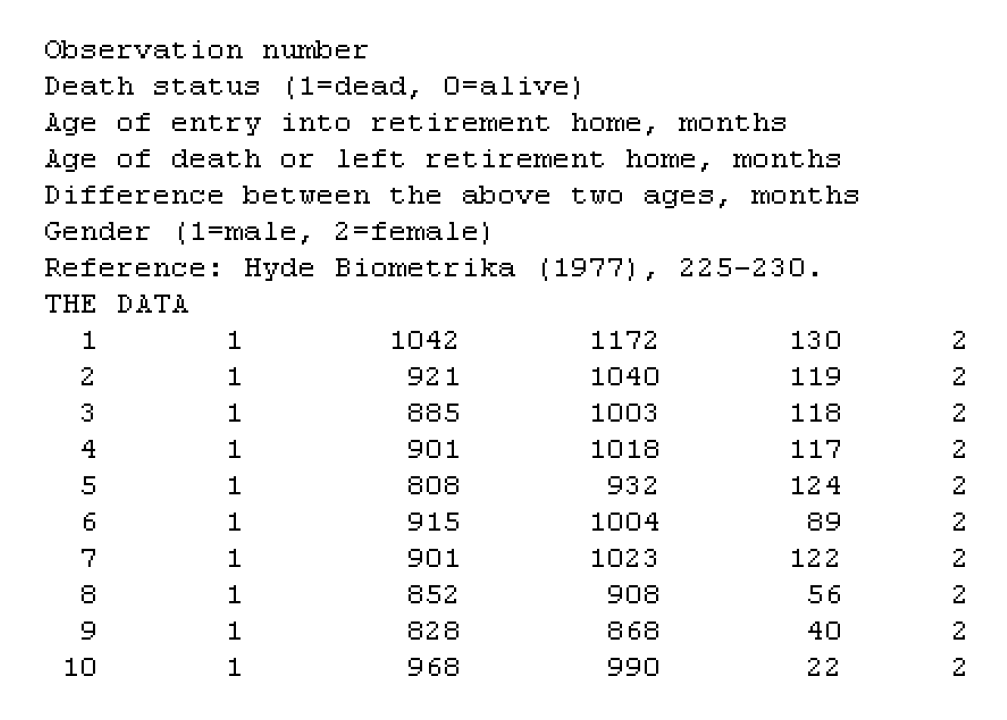
\includegraphics[width=0.4\linewidth,height=\textheight,keepaspectratio]{figura/ejemp3.png}
\end{center}

\begin{center}\rule{0.5\linewidth}{0.5pt}\end{center}

\subsubsection{Ejemplo Tiempo al primer uso de
marihuana.}\label{ejemplo-tiempo-al-primer-uso-de-marihuana.}

\begin{quote}
En este estudio a 191 estudiantes de preparatoria se les preguntó: ¿Cuál
fue la primera vez que probaste la marihuana?. Las respuestas fueron,
``la edad exacta a la que la probaron'', ``nunca la he probado'', y ``la
probé pero no recuerdo cuando fue la primera vez''. En este último caso
tenemos una censura por la izquierda. El evento de interés ha ocurrido
en algún momento previo a la edad actual del estudiante!.
\end{quote}

\begin{center}
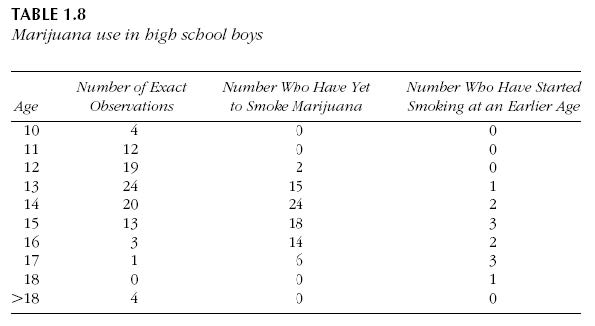
\includegraphics[width=5in,height=\textheight,keepaspectratio]{figura/ejemp4.jpg}
\end{center}

\begin{center}\rule{0.5\linewidth}{0.5pt}\end{center}

\subsubsection{Tiempo a desarrollar
sida.}\label{tiempo-a-desarrollar-sida.}

\begin{quote}
Se reportan datos con tiempos de infección y de inducción para 258
adultos y 37 niños que fueron infectados con el virus del VIH y
desarrollaron sida antes del 30 de junio de 1986. Los datos consisten de
los tiempos (en años) desde que adultos fueron infectados por el virus
por transfusión de sangre contaminada, y el tiempo de espera hasta el
desarrollo de sida. Para la población pediátrica, los niños fueron
infectados en útero o al nacer. El tiempo base de medición es el 1 de
abril de 1978. En este estudio, sólo los individuos que han desarrollado
sida antes del término del estudio son considerados. Individuos que no
han desarrollado sida no son incluidos en el estudio. Este tipo de datos
es llamado truncados por la derecha y más adelante los veremos con
detalle.
\end{quote}

\subsubsection{Tiempo de inducción de SIDA en adultos y
niños}\label{tiempo-de-inducciuxf3n-de-sida-en-adultos-y-niuxf1os}

\begin{longtable}[]{@{}
  >{\raggedright\arraybackslash}p{(\linewidth - 4\tabcolsep) * \real{0.2319}}
  >{\raggedright\arraybackslash}p{(\linewidth - 4\tabcolsep) * \real{0.4493}}
  >{\raggedright\arraybackslash}p{(\linewidth - 4\tabcolsep) * \real{0.3188}}@{}}
\toprule\noalign{}
\begin{minipage}[b]{\linewidth}\raggedright
Infection Time
\end{minipage} & \begin{minipage}[b]{\linewidth}\raggedright
Adult Induction Time
\end{minipage} & \begin{minipage}[b]{\linewidth}\raggedright
Child Induction Time
\end{minipage} \\
\midrule\noalign{}
\endhead
\bottomrule\noalign{}
\endlastfoot
0.00 & 5 & \\
0.25 & 6.75 & \\
0.75 & 5, 5, 7.25 & \\
1.00 & 4.25, 5.75, 6.25, 6.5 & 5.5 \\
1.25 & 4, 4.25, 4.75, 5.75 & \\
1.50 & 2.75, 3.75, 5, 5.5, 6.5 & 2.25 \\
1.75 & 2.75, 3, 5.25, 5.25 & \\
2.00 & 2.25, 3, 4, 4.5, 4.75, 5, \ldots{} & \\
2.25 & 3, 5.5 & 3 \\
2.50 & 2.25, 2.25, \ldots, 4 & \\
2.75 & 1.25, 1.5, \ldots, 5.25 & 1 \\
3.00 & 2, 3.25, \ldots, 5 & 1.75 \\
3.25 & 1.25, 1.75, \ldots, 4.5 & \\
3.50 & 1.25, 2.25, \ldots, 4.5 & 0.75 \\
3.75 & 1.25, 1.75, \ldots, 4.25 & 0.75, 1, \ldots, 4.25 \\
4.00 & 1, 1.5, \ldots, 4 & 1 \\
4.25 & 1.25, 1.5, \ldots, 3.5 & 1.75 \\
4.50 & 1, 1.5, \ldots, 3.25 & 3.25 \\
4.75 & 1, 1.5, \ldots, 3.25 & 1, 2.25 \\
5.00 & 0.5, 1.5, \ldots, 3 & 0.5, 0.75, 1.5, 2.5 \\
5.25 & 0.25, 0.25, \ldots, 2.75 & 0.25, 1, 1.5 \\
5.50 & 1, 1, \ldots, 2.5 & 0.5, 1.5, 2.5 \\
5.75 & 0.25, 0.75, \ldots, 2.25 & 1.75 \\
6.00 & 0.5, 0.75, \ldots, 2 & 0.5, 1.25 \\
6.25 & 0.75, 1, \ldots, 1.75 & 0.5, 1.25 \\
6.50 & 0.25, 0.25, \ldots, 1.5 & 0.75 \\
6.75 & 0.75, 0.75, \ldots, 1.25 & 0.5, 0.75 \\
7.00 & 0.75 & 0.75 \\
7.25 & 0.25 & 0.25 \\
\end{longtable}

\begin{center}\rule{0.5\linewidth}{0.5pt}\end{center}

\subsection{Ejemplo de datos
simulados}\label{ejemplo-de-datos-simulados}

\begin{Shaded}
\begin{Highlighting}[]
\CommentTok{\# Ejemplo simulado de tiempos de supervivencia}
\FunctionTok{set.seed}\NormalTok{(}\DecValTok{123}\NormalTok{)}
\NormalTok{tiempos }\OtherTok{\textless{}{-}} \FunctionTok{rexp}\NormalTok{(}\DecValTok{8}\NormalTok{, }\AttributeTok{rate =} \FloatTok{0.05}\NormalTok{)}
\NormalTok{status }\OtherTok{\textless{}{-}} \FunctionTok{rbinom}\NormalTok{(}\DecValTok{8}\NormalTok{, }\DecValTok{1}\NormalTok{, }\AttributeTok{prob =} \FloatTok{0.8}\NormalTok{)}
\FunctionTok{library}\NormalTok{(survival)}
\NormalTok{data\_sim }\OtherTok{\textless{}{-}} \FunctionTok{data.frame}\NormalTok{(}\AttributeTok{time =}\NormalTok{ tiempos, }\AttributeTok{event =}\NormalTok{ status)}
\end{Highlighting}
\end{Shaded}

\begin{longtable}[]{@{}rr@{}}
\caption{Primeros 8 registros de data\_sim}\tabularnewline
\toprule\noalign{}
time & event \\
\midrule\noalign{}
\endfirsthead
\toprule\noalign{}
time & event \\
\midrule\noalign{}
\endhead
\bottomrule\noalign{}
\endlastfoot
16.8691452 & 1 \\
11.5322054 & 0 \\
26.5810974 & 1 \\
0.6315472 & 1 \\
1.1242195 & 1 \\
6.3300243 & 0 \\
6.2845458 & 0 \\
2.9053361 & 1 \\
\end{longtable}

\section{Tipos de datos: eventos, censura,
truncamiento}\label{tipos-de-datos-eventos-censura-truncamiento}

\subsection{Censura y truncamiento}\label{sec-censura-y-truncamiento}

\subsubsection{\texorpdfstring{¿Qué es la
\textbf{censura}?}{¿Qué es la censura?}}\label{quuxe9-es-la-censura}

\begin{itemize}
\tightlist
\item
  La \textbf{censura} ocurre cuando \textbf{no se observa completamente}
  el tiempo de fallo.
\item
  Es común en estudios longitudinales, donde algunos individuos:

  \begin{itemize}
  \tightlist
  \item
    \textbf{No han fallado} al final del estudio,
  \item
    \textbf{Ingresan tarde} al seguimiento,
  \item
    O \textbf{se pierde el seguimiento}.
  \end{itemize}
\end{itemize}

\textbf{Tipos de censura}:

\begin{itemize}
\tightlist
\item
  \textbf{Por la derecha}: solo sabemos que el evento ocurrió después de
  cierto tiempo.
\item
  \textbf{Por la izquierda}: solo sabemos que ocurrió antes de cierto
  tiempo.
\item
  \textbf{Por intervalo}: solo sabemos que ocurrió entre dos tiempos.
\end{itemize}

\subsubsection{\texorpdfstring{¿Qué es el
\textbf{truncamiento}?}{¿Qué es el truncamiento?}}\label{quuxe9-es-el-truncamiento}

\begin{itemize}
\tightlist
\item
  El \textbf{truncamiento} ocurre cuando \textbf{ciertas observaciones
  nunca se registran} debido al diseño del estudio.
\end{itemize}

\textbf{Ejemplos}:

\begin{itemize}
\tightlist
\item
  \textbf{Truncamiento por la izquierda}: sólo se incluyen individuos
  cuyo evento ocurre \textbf{después} de cierto punto.
\item
  \textbf{Truncamiento por la derecha}: se excluyen individuos cuyo
  evento ocurre \textbf{después} de cierto punto.
\end{itemize}

\textbf{Implicación}:

\begin{itemize}
\tightlist
\item
  Afecta \textbf{quién entra al estudio} (selección), no solo cómo se
  mide el tiempo.
\end{itemize}

\begin{center}\rule{0.5\linewidth}{0.5pt}\end{center}

\subsection{Tipos de censura por la
derecha}\label{tipos-de-censura-por-la-derecha}

\subsubsection{¿Cómo se genera la
censura?}\label{cuxf3mo-se-genera-la-censura}

En estudios de supervivencia, es común que \textbf{no se observe
completamente} el tiempo de falla. Esto ocurre mediante distintos
mecanismos:

\begin{itemize}
\tightlist
\item
  \textbf{Censura tipo I}
\item
  \textbf{Censura tipo II}
\item
  \textbf{Censura aleatoria}
\end{itemize}

\begin{center}\rule{0.5\linewidth}{0.5pt}\end{center}

\subsection{Censura tipo I}\label{censura-tipo-i}

\textbf{Definición}:\\
Se observa el tiempo de supervivencia \(T_i\) \textbf{solo si ocurre
antes de un tiempo de censura predeterminado} \(C_i\).\\
Si \(T_i > C_i\), entonces el dato está censurado.

\textbf{Notación formal}:

\begin{itemize}
\tightlist
\item
  Observamos el par \((t_i, \delta_i)\), donde

  \begin{itemize}
  \tightlist
  \item
    \(t_i = \min(T_i, C_i)\)\\
  \item
    \(\delta_i = I(T_i \le C_i)\)\\
  \end{itemize}
\item
  Si \(\delta_i = 1\): observación completa\\
\item
  Si \(\delta_i = 0\): censura por la derecha
\end{itemize}

\begin{center}
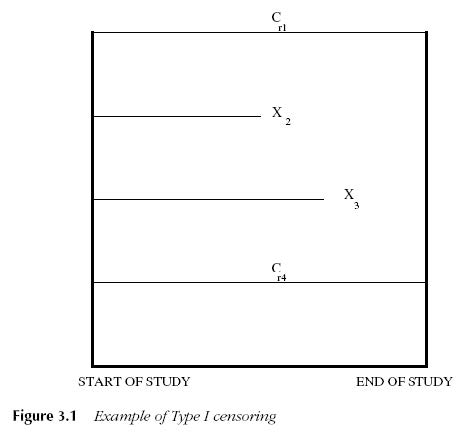
\includegraphics[width=0.9\linewidth,height=\textheight,keepaspectratio]{figura/CensuraI.jpg}
\end{center}

\begin{center}\rule{0.5\linewidth}{0.5pt}\end{center}

\subsubsection{Ejemplo de censura tipo
I}\label{ejemplo-de-censura-tipo-i}

\begin{quote}
En un estudio toxicológico, ratones reciben un carcinógeno.\\
Se observa su supervivencia hasta cierto tiempo límite.\\
Los ratones aún vivos en ese punto son sacrificados (censurados).
\end{quote}

\textbf{Importante}: Puede haber \textbf{múltiples tiempos de censura},
dependiendo del diseño experimental.

\begin{center}
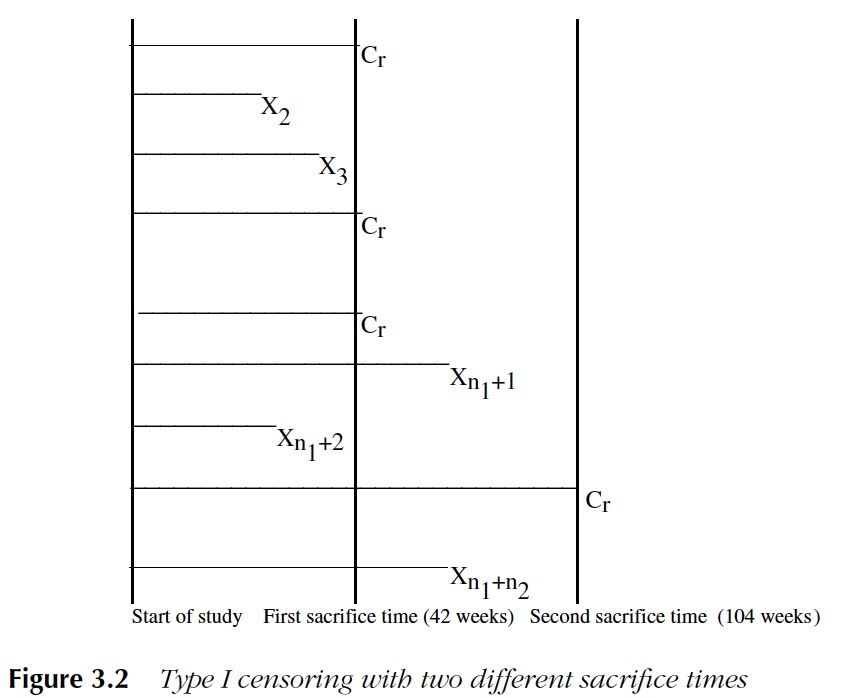
\includegraphics[width=0.9\linewidth,height=\textheight,keepaspectratio]{figura/CensuraI-3.jpg}
\end{center}

\begin{center}\rule{0.5\linewidth}{0.5pt}\end{center}

\subsubsection{Censura tipo I
generalizada}\label{censura-tipo-i-generalizada}

\begin{quote}
Cada individuo entra en un momento distinto al estudio, pero el final
del estudio está predeterminado.
\end{quote}

\begin{itemize}
\tightlist
\item
  Cada sujeto tiene su propio tiempo de censura fijo.
\item
  Este diseño genera \textbf{censura tipo I generalizada}.
\end{itemize}

\begin{center}
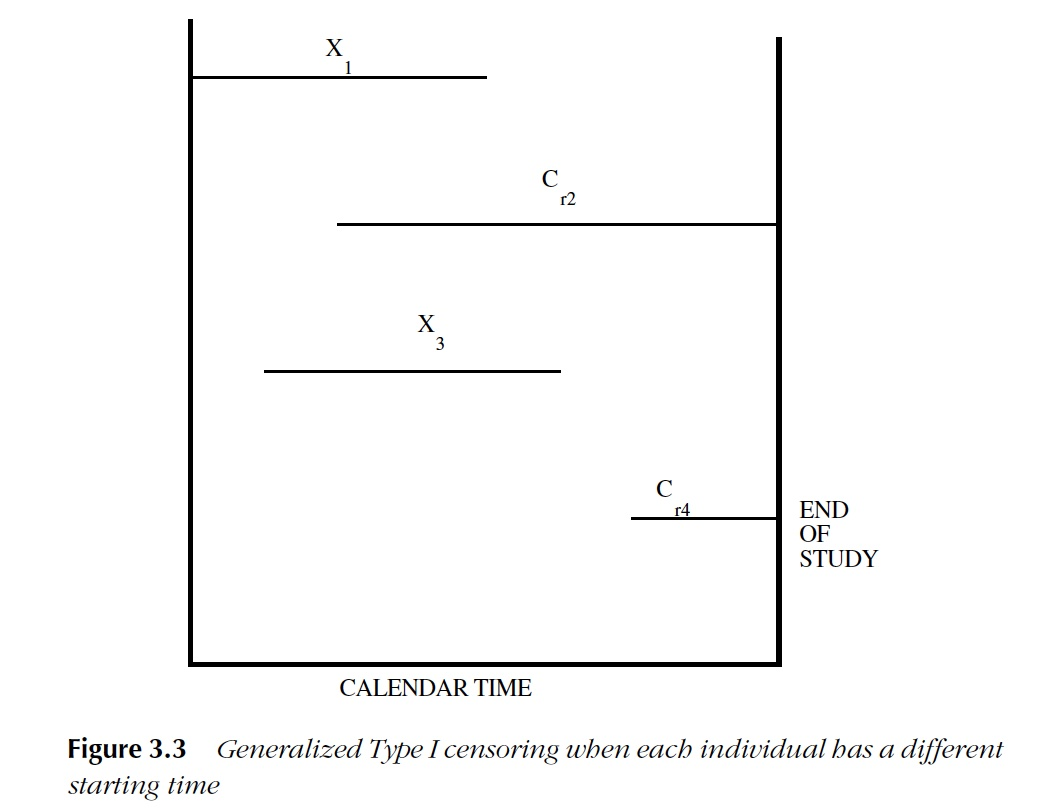
\includegraphics[width=1\linewidth,height=\textheight,keepaspectratio]{figura/CensuraI-2.jpg}
\end{center}

\begin{center}\rule{0.5\linewidth}{0.5pt}\end{center}

\subsection{Censura tipo II}\label{censura-tipo-ii}

\textbf{Definición}:\\
El estudio se \textbf{detiene al observar la falla de los primeros}
\(r < n\) sujetos.

\begin{itemize}
\tightlist
\item
  Se observan los tiempos \(T_{(1)}, T_{(2)}, \dots, T_{(r)}\)
\item
  Los \(n - r\) sujetos restantes están censurados.
\end{itemize}

\textbf{Notación}:

\begin{itemize}
\tightlist
\item
  Tiempo de censura común: \(C = T_{(r)}\)
\item
  Censura si \(T_i > C\)
\end{itemize}

\emph{Aplicación típica}: pruebas de resistencia de equipos que se
detienen al fallar cierto número de unidades.

\emph{Ejemplo}: Se prueban 10 motores, pero se termina el estudio tras
la falla de los primeros 5.

\pandocbounded{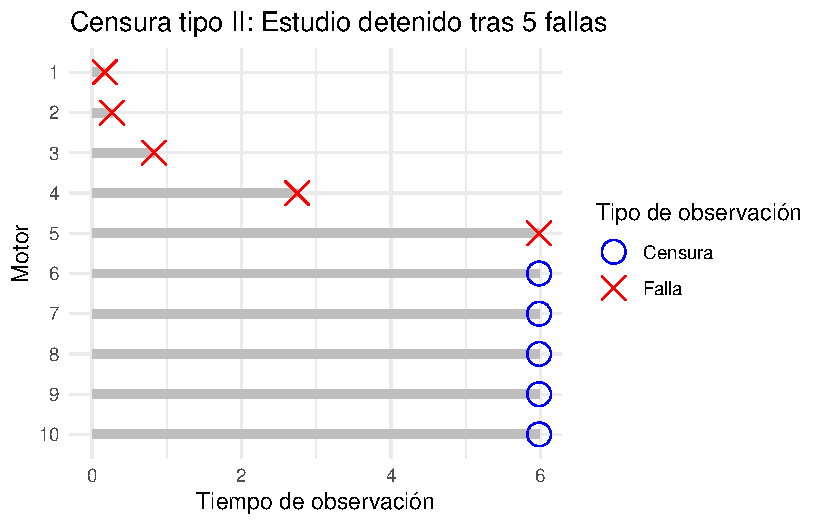
\includegraphics[keepaspectratio]{Unidad1_files/figure-pdf/unnamed-chunk-4-1.pdf}}

\begin{center}\rule{0.5\linewidth}{0.5pt}\end{center}

\subsection{Censura aleatoria}\label{censura-aleatoria}

\textbf{Definición}:\\
El tiempo de censura \(C_i\) es una \textbf{variable aleatoria},
diferente para cada individuo.

\textbf{Ejemplos comunes}:

\begin{itemize}
\tightlist
\item
  Salida del estudio
\item
  Muerte por otra causa
\item
  Migración o pérdida de contacto
\item
  Hospital deja de aceptar al paciente
\end{itemize}

\emph{Ejemplo aplicado}:

\begin{quote}
En estudios con pacientes de diálisis, el evento de interés puede ser
fallas por infección, pero se censura por muerte o salida del hospital.
\end{quote}

\subsubsection{Tipos de censura
aleatoria}\label{tipos-de-censura-aleatoria}

\begin{itemize}
\tightlist
\item
  \textbf{No informativa}: \(C_i \perp T_i\)\\
  → tratable como censura tipo I
\item
  \textbf{Informativa}: \(C_i\) depende de \(T_i\)\\
  → requiere modelos avanzados
\end{itemize}

\begin{center}\rule{0.5\linewidth}{0.5pt}\end{center}

\subsection{Censura por la izquierda e
intervalo}\label{censura-por-la-izquierda-e-intervalo}

\subsubsection{¿Qué es la censura por la
izquierda?}\label{quuxe9-es-la-censura-por-la-izquierda}

\begin{itemize}
\tightlist
\item
  Ocurre cuando \textbf{el evento de interés sucede antes de un tiempo
  de observación conocido}.
\item
  Es decir, \textbf{sabemos que el evento ya ocurrió}, pero \textbf{no
  cuándo exactamente}.
\end{itemize}

\textbf{Definición formal}:\\
Sea \(C_l\) el tiempo de censura por la izquierda y \(T_i\) el tiempo de
falla.

\begin{itemize}
\tightlist
\item
  Si \(T_i \ge C_l\): observación completa.\\
\item
  Si \(T_i < C_l\): \textbf{censura por la izquierda}.
\end{itemize}

\textbf{Notación}:\\
\[
t_i = \max(T_i, C_l), \quad 
\delta_i = I(T_i \ge C_l)
\]

\textbf{Ejemplo 1}

\begin{quote}
Adolescente declara:\\
\emph{``Sí consumí marihuana, pero no recuerdo cuándo''.}\\
→ El evento ocurrió antes de su edad actual, pero se desconoce el
momento exacto.
\end{quote}

\textbf{Ejemplo 2}

\begin{quote}
Un niño ya sabe realizar una tarea cuando entra al estudio.\\
→ El aprendizaje ocurrió antes de la observación inicial.
\end{quote}

\begin{center}\rule{0.5\linewidth}{0.5pt}\end{center}

\subsection{Censura doble (izquierda y
derecha)}\label{censura-doble-izquierda-y-derecha}

\textbf{Definición}:\\
Una observación está \textbf{doblemente censurada} si se desconoce si el
evento ocurrió antes o después de un cierto rango.

\begin{itemize}
\tightlist
\item
  Combina censura por la izquierda y la derecha.
\item
  Común en estudios transversales o con límites temporales de
  observación.
\end{itemize}

\textbf{Notación generalizada}:

\[
t_i = \max\{ \min(T_i, C_r), C_l \}, \quad
\delta_i =
\begin{cases}
1, & \text{tiempo exacto} \\
0, & \text{censura por la derecha} \\
-1, & \text{censura por la izquierda}
\end{cases}
\]

\textbf{Ejemplo 1 -- Marihuana}

\begin{quote}
``Nunca la he usado'' → censura por la derecha\\
``Sí la usé pero no recuerdo cuándo'' → izquierda\\
``La usé a los 15'' → observación completa
\end{quote}

\textbf{Ejemplo 2 -- Aprendizaje infantil}

\begin{quote}
Algunos niños no aprenden durante el estudio → censura por la derecha\\
Otros ya sabían antes de iniciar → censura por la izquierda
\end{quote}

\begin{center}\rule{0.5\linewidth}{0.5pt}\end{center}

\subsection{Comparación}\label{comparaciuxf3n}

\begin{longtable}[]{@{}
  >{\raggedright\arraybackslash}p{(\linewidth - 2\tabcolsep) * \real{0.5000}}
  >{\raggedright\arraybackslash}p{(\linewidth - 2\tabcolsep) * \real{0.5000}}@{}}
\toprule\noalign{}
\begin{minipage}[b]{\linewidth}\raggedright
Tipo de observación
\end{minipage} & \begin{minipage}[b]{\linewidth}\raggedright
Línea de tiempo
\end{minipage} \\
\midrule\noalign{}
\endhead
\bottomrule\noalign{}
\endlastfoot
\textbf{Exacta} & Evento ocurre entre observación inicial y final \\
\textbf{Censura por la derecha} & Línea que termina sin evento
registrado \\
\textbf{Censura por la izquierda} & Línea que empieza con evento ya
ocurrido \\
\textbf{Doble censura} & Solo se sabe que el evento ocurrió fuera del
intervalo de observación \\
\end{longtable}

\pandocbounded{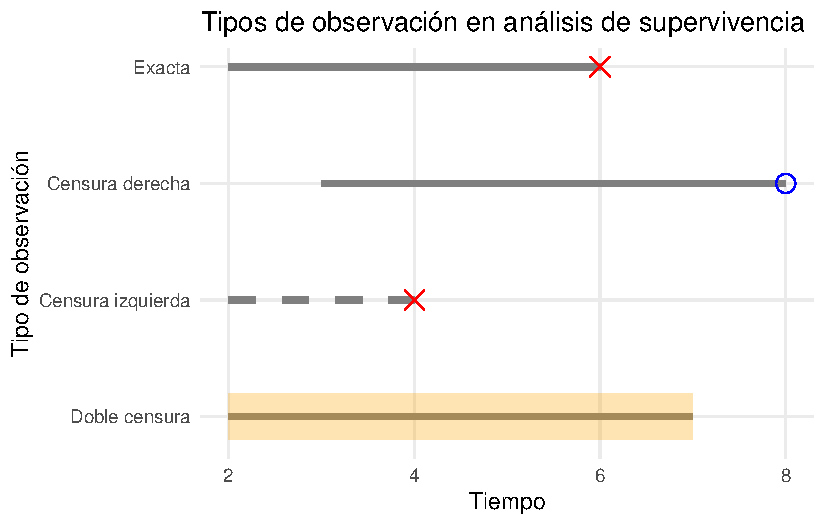
\includegraphics[keepaspectratio]{Unidad1_files/figure-pdf/unnamed-chunk-5-1.pdf}}

\begin{center}\rule{0.5\linewidth}{0.5pt}\end{center}

\subsection{Recomendaciones}\label{recomendaciones}

\begin{itemize}
\tightlist
\item
  Identificar con claridad el \textbf{momento de entrada} al estudio y
  el \textbf{horizonte de observación}.
\item
  Siempre registrar \textbf{si se trata de censura por la izquierda,
  derecha o ambas}.
\item
  Verificar si la censura es \textbf{informativa o no informativa}.
\end{itemize}

\subsection{Censura por intervalo}\label{censura-por-intervalo}

\subsubsection{¿Qué es la censura por
intervalo?}\label{quuxe9-es-la-censura-por-intervalo}

\begin{itemize}
\tightlist
\item
  La \textbf{censura por intervalo} ocurre cuando \textbf{el evento
  sucede entre dos visitas clínicas}, pero \textbf{no se conoce el
  momento exacto}.
\end{itemize}

\textbf{Interpretación}:\\
Se sabe que el sujeto \textbf{no había fallado antes del tiempo}
\(L_i\), pero sí \textbf{lo ha hecho antes o en el tiempo} \(R_i\).

\textbf{Notación formal}:

\[
L_i < T_i \le R_i
\]

Donde:

\begin{itemize}
\tightlist
\item
  \(L_i\) = última vez que se observó sin evento\\
\item
  \(R_i\) = primera vez que se detecta el evento
\end{itemize}

Puedes pensar esta censura como una observación \textbf{con ventana de
tiempo}, en la que el evento ocurre \textbf{dentro de un intervalo} que
puede variar por sujeto.

Posibles causas:

\begin{itemize}
\tightlist
\item
  Visitas clínicas programadas
\item
  Limitaciones de seguimiento continuo
\end{itemize}

\begin{center}\rule{0.5\linewidth}{0.5pt}\end{center}

\subsubsection{Ejemplo 1 -- Estudio del Corazón de
Framingham}\label{ejemplo-1-estudio-del-corazuxf3n-de-framingham}

\begin{quote}
En este estudio longitudinal, los eventos de enfermedad coronaria (CHD)
pueden registrarse con precisión.
\end{quote}

Sin embargo:

\begin{itemize}
\tightlist
\item
  La aparición de \textbf{angina de pecho} se detecta solo \textbf{entre
  dos visitas clínicas}, con varios años de diferencia.
\end{itemize}

→ El tiempo exacto es desconocido, pero \textbf{ocurrió dentro del
intervalo} entre exámenes.

\begin{center}\rule{0.5\linewidth}{0.5pt}\end{center}

\subsubsection{Ejemplo 2 -- Estudio de
radioterapia}\label{ejemplo-2-estudio-de-radioterapia}

\begin{quote}
Se estudió el efecto cosmético en mujeres con cáncer de mama tras
radioterapia (con o sin quimioterapia).
\end{quote}

\begin{itemize}
\tightlist
\item
  Se realizaron controles \textbf{cada 4 a 6 meses}, luego más
  espaciados.
\item
  El evento de interés: \textbf{retracción severa del seno}.
\item
  Solo se sabía si \textbf{ocurrió entre dos visitas}, o si
  \textbf{nunca se observó} (censura por la derecha).
\end{itemize}

→ Algunas pacientes presentaron \textbf{censura por intervalo}, y otras,
\textbf{por la derecha}.

\begin{center}\rule{0.5\linewidth}{0.5pt}\end{center}

\subsubsection{Actividad: Identificación y análisis de datos de
supervivencia}\label{actividad-identificaciuxf3n-y-anuxe1lisis-de-datos-de-supervivencia}

\paragraph{Objetivo}\label{objetivo}

Aplicar los conceptos fundamentales del análisis de supervivencia
identificando un conjunto de datos relevante, describiendo su estructura
temporal, y evaluando la presencia y tipo de censura.

\paragraph{Instrucciones}\label{instrucciones}

\begin{enumerate}
\def\labelenumi{\arabic{enumi}.}
\item
  \textbf{Buscar o seleccionar un conjunto de datos} que permita aplicar
  análisis de supervivencia. Puede ser:

  \begin{itemize}
  \tightlist
  \item
    Un conjunto de datos \textbf{propio} (proyecto, tesis, trabajo
    profesional).
  \item
    Un conjunto de datos \textbf{público} (Kaggle, UCI, CRAN, etc.).
  \end{itemize}
\item
  \textbf{Describir el contexto del estudio}, incluyendo:

  \begin{itemize}
  \tightlist
  \item
    La \textbf{unidad de análisis} (por ejemplo: paciente, máquina,
    usuario).
  \item
    La \textbf{variable de tiempo} (por ejemplo: días hasta falla,
    semanas hasta abandono).
  \item
    El \textbf{evento de interés} (por ejemplo: muerte, falla, compra,
    abandono).
  \end{itemize}
\item
  \textbf{Explicar la estructura temporal del estudio}, atendiendo a las
  siguientes recomendaciones:

  \begin{itemize}
  \tightlist
  \item
    Identificar con claridad el \textbf{momento de entrada} al estudio y
    el \textbf{horizonte de observación}.
  \item
    Registrar si se trata de \textbf{censura por la izquierda, derecha o
    ambas}.
  \item
    Verificar si la censura es \textbf{informativa o no informativa}.
  \end{itemize}
\item
  \textbf{Entregar un breve reporte (1-2 cuartillas)} que contenga:

  \begin{itemize}
  \tightlist
  \item
    Descripción del conjunto de datos.
  \item
    Contexto del estudio y definición del evento.
  \item
    Discusión sobre tipo(s) de censura y su naturaleza.
  \item
    Una tabla ilustrativa con al menos 10 observaciones con las
    columnas: \texttt{ID}, \texttt{tiempo}, \texttt{status} (evento = 1,
    censura = 0).
  \end{itemize}
\end{enumerate}

\begin{center}\rule{0.5\linewidth}{0.5pt}\end{center}

\subsection{Truncamiento}\label{truncamiento}

\subsubsection{¿Qué es el
truncamiento?}\label{quuxe9-es-el-truncamiento-1}

\begin{itemize}
\tightlist
\item
  El \textbf{truncamiento} ocurre cuando \textbf{ciertos individuos no
  aparecen en el estudio}, porque \textbf{su tiempo de falla está fuera
  de una ventana de observación}.
\end{itemize}

\textbf{Diferencia clave con la censura}:

\begin{itemize}
\tightlist
\item
  \textbf{Censura} → se observa parcialmente
\item
  \textbf{Truncamiento} → \textbf{no se observa en absoluto}
\end{itemize}

\textbf{Definición formal}:\\
Se observa \(T_i\) \textbf{solo si} \(T_i \in (U_i, V_i)\)

\emph{Imaginemos una ventana de observación:}\\
Si el evento ocurre \textbf{antes} de entrar a la ventana o
\textbf{después de que cierra}, el sujeto \textbf{no entra al estudio}.

Esto es \textbf{truncamiento}, no censura.

\begin{center}\rule{0.5\linewidth}{0.5pt}\end{center}

\subsection{Truncamiento por la
izquierda}\label{truncamiento-por-la-izquierda}

\textbf{Definición}:\\
Solo se observan individuos cuyo tiempo de evento \textbf{supera un
umbral inferior}:\\
\[
T_i > U_i
\]

También conocido como \textbf{entrada retardada}: el sujeto
\textbf{debió sobrevivir} lo suficiente para entrar al estudio.

\begin{quote}
\textbf{Ejemplo -- Centro de retiro}\\
En Channing House, solo se estudian residentes que \textbf{lograron
ingresar}.\\
Quienes murieron \textbf{antes} de tener edad para ingresar, \textbf{no
aparecen} en el estudio.\\
→ \textbf{Truncamiento por la izquierda}
\end{quote}

\begin{center}\rule{0.5\linewidth}{0.5pt}\end{center}

\subsection{Truncamiento por la
derecha}\label{truncamiento-por-la-derecha}

\textbf{Definición}:\\
Solo se incluyen sujetos cuyo evento ocurre \textbf{antes de un umbral
superior}: \[
T_i < V_i
\]

Esto puede ocurrir en \textbf{estudios retrospectivos con fecha de
corte}.

\begin{quote}
\textbf{Ejemplo -- Estudio del SIDA}\\
Solo se incluyen pacientes que desarrollaron SIDA \textbf{antes del 30
de junio de 1986}.\\
Aquellos cuya enfermedad apareció después, \textbf{no fueron
observados}.\\
→ \textbf{Truncamiento por la derecha}
\end{quote}

\begin{center}\rule{0.5\linewidth}{0.5pt}\end{center}

\subsection{Truncamiento y censura
combinados}\label{truncamiento-y-censura-combinados}

\begin{itemize}
\item
  Es \textbf{común} que los estudios de supervivencia combinen:

  \begin{itemize}
  \tightlist
  \item
    \textbf{Truncamiento por la izquierda} (entrada tardía)
  \item
    \textbf{Censura por la derecha} (seguimiento limitado)
  \end{itemize}
\item
  Ejemplo típico:

  \begin{quote}
  Un paciente entra al estudio tras cumplir ciertos criterios
  (truncamiento),\\
  pero el estudio termina antes de que fallezca (censura).
  \end{quote}
\end{itemize}

\section{Visualización}\label{visualizaciuxf3n}

\subsection{Ejemplo: Ensayo clínico con
cáncer}\label{ejemplo-ensayo-cluxednico-con-cuxe1ncer}

\begin{longtable}[]{@{}rrrr@{}}
\toprule\noalign{}
paciente & entrada & fin & evento \\
\midrule\noalign{}
\endhead
\bottomrule\noalign{}
\endlastfoot
1 & 2000 & 2007 & 0 \\
2 & 2000 & 2006 & 1 \\
3 & 2001 & 2007 & 0 \\
4 & 2002 & 2007 & 0 \\
5 & 2002 & 2004 & 1 \\
6 & 2002 & 2006 & 1 \\
\end{longtable}

\begin{figure}[H]

{\centering \pandocbounded{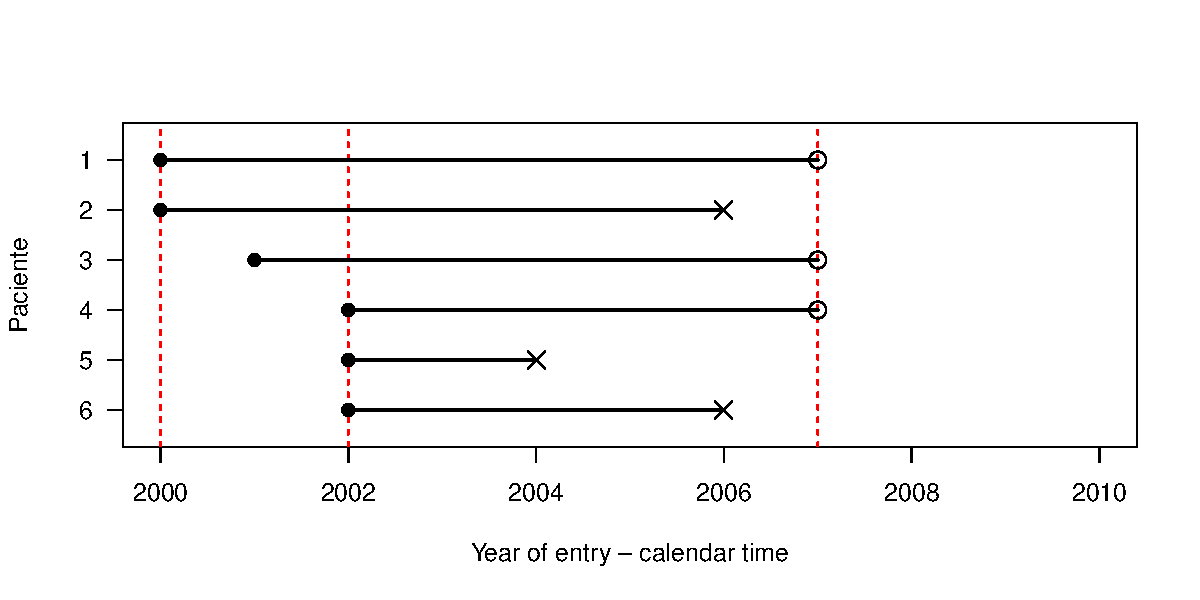
\includegraphics[keepaspectratio]{Unidad1_files/figure-pdf/unnamed-chunk-8-1.pdf}}

}

\caption{Reclutamiento y seguimiento}

\end{figure}%

\begin{center}\rule{0.5\linewidth}{0.5pt}\end{center}

\subsection{Representación gráfica del
seguimiento}\label{representaciuxf3n-gruxe1fica-del-seguimiento}

\begin{longtable}[]{@{}rrr@{}}
\caption{Ejemplo}\tabularnewline
\toprule\noalign{}
paciente & tiempo & status \\
\midrule\noalign{}
\endfirsthead
\toprule\noalign{}
paciente & tiempo & status \\
\midrule\noalign{}
\endhead
\bottomrule\noalign{}
\endlastfoot
1 & 7 & 0 \\
2 & 6 & 1 \\
3 & 6 & 0 \\
4 & 5 & 0 \\
5 & 2 & 1 \\
6 & 4 & 1 \\
\end{longtable}

\begin{itemize}
\tightlist
\item
  Círculo abierto = censura
\item
  X = evento (muerte)
\end{itemize}

\begin{figure}

\begin{minipage}{\linewidth}
\pandocbounded{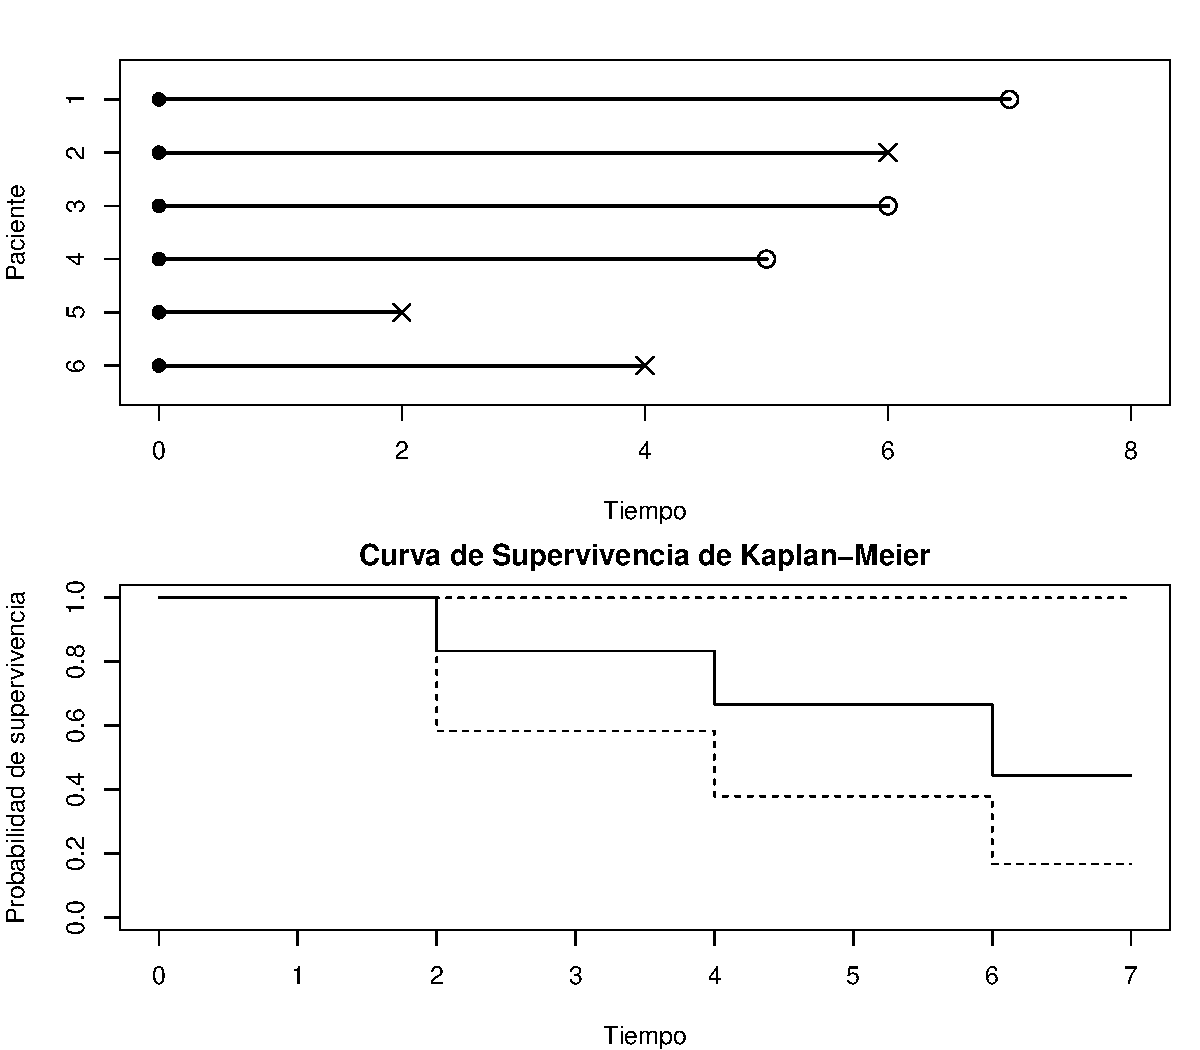
\includegraphics[keepaspectratio]{Unidad1_files/figure-pdf/unnamed-chunk-10-1.pdf}}\end{minipage}%

\end{figure}%

\begin{center}\rule{0.5\linewidth}{0.5pt}\end{center}

\subsection{Visualización de
data\_sim}\label{visualizaciuxf3n-de-data_sim}

\pandocbounded{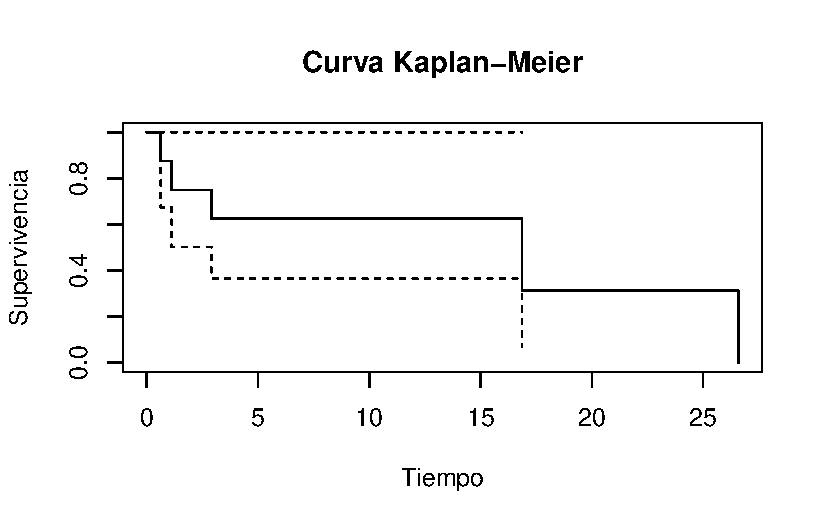
\includegraphics[keepaspectratio]{Unidad1_files/figure-pdf/unnamed-chunk-11-1.pdf}}

\section{Referencias}\label{referencias}

\phantomsection\label{refs}
\begin{CSLReferences}{1}{0}
\bibitem[\citeproctext]{ref-klein2003}
Klein, J. P., \& Moeschberger, M. L. (2003). \emph{Survival analysis:
Techniques for censored and truncated data} (2nd ed.). Springer.

\end{CSLReferences}




\end{document}
